\documentclass{beamer}
\usefonttheme[onlymath]{serif}
\usepackage[T1]{fontenc}
\usepackage[utf8]{inputenc}
\usepackage[english]{babel}
\usepackage{amsmath}
\usepackage{amssymb}
\usepackage{amsthm}
\usepackage{gensymb}
\usepackage{parskip}
\usepackage{mathtools}
\usepackage{listings}
\usepackage{hyperref}
\usepackage{graphicx}
\usepackage{color}
\usepackage{enumerate}
\usepackage{tikz}
\usetikzlibrary{calc}
\usetikzlibrary{positioning}
\usetikzlibrary{angles}
\usetikzlibrary{shapes}
\usetikzlibrary{arrows}
\usepackage{verbatim}
\usepackage{multicol}
\usepackage{array}
\usepackage{minted}
\parskip 0pt

\usepackage{colortbl}
\usepackage{pgf}
\usepackage{pgfkeys}
\usetikzlibrary{fpu}
\usepackage{tkz-euclide}

\DeclareMathOperator{\lcm}{lcm}
\newcommand\floor[1]{\left\lfloor#1\right\rfloor}
\newcommand\ceil[1]{\left\lceil#1\right\rceil}
\newcommand\abs[1]{\left|#1\right|}
\newcommand\p[1]{\left(#1\right)}
\newcommand\sqp[1]{\left[#1\right]}
\newcommand\cp[1]{\left\{#1\right\}}
\newcommand\norm[1]{\left\lVert#1\right\rVert}
\renewcommand\Im{\operatorname{Im}}
\renewcommand\Re{\operatorname{Re}}

\usetheme{metropolis}
\definecolor{dark yellow}{rgb} {0.6,0.6,0.0}
\definecolor{dark green}{rgb} {0.0,0.6,0.0}

\graphicspath{{myndir/}}

\tikzstyle{vertex}=[circle,fill=black!50,minimum size=15pt,inner sep=0pt, font=\small]
\tikzstyle{selected vertex} = [vertex, fill=red!24]
\tikzstyle{edge} = [draw,thick,-]
\tikzstyle{dedge} = [draw,thick,->]
\tikzstyle{weight} = [font=\scriptsize,pos=0.5]
\tikzstyle{selected edge} = [draw,line width=2pt,-,red!50]
\tikzstyle{selected2 vertex} = [vertex, fill=hilight!50, text=black]
\tikzstyle{ignored edge} = [draw,line width=5pt,-,black!20]
\tikzstyle{vertex1} = [vertex, fill=red]
\tikzstyle{vertex2} = [vertex, fill=blue]
\tikzstyle{vertex3} = [vertex, fill=green, text=black]
\tikzstyle{vertex4} = [vertex, fill=yellow, text=black]
\tikzstyle{vertex5} = [vertex, fill=pink, text=black]
\tikzstyle{vertex6} = [vertex, fill=purple]

\tikzset{
  treenode/.style = {align=center, inner sep=0pt, text centered,
    font=\sffamily},
  vertex/.style = {treenode, circle, black, font=\sffamily\bfseries\tiny, draw=black, text width=1.8em},% arbre rouge noir, noeud noir
  rvertex/.style = {treenode, circle, black, font=\sffamily\bfseries\tiny, draw=red, text width=1.8em},% arbre rouge noir, noeud noir
}

\definecolor{offwhite}{RGB}{249,242,215}
\definecolor{foreground}{HTML}{23373b}
\definecolor{background}{RGB}{24,24,24}
\definecolor{title}{RGB}{107,174,214}
\definecolor{gray}{RGB}{155,155,155}
\definecolor{subtitle}{RGB}{102,255,204}
\definecolor{lolight}{RGB}{155,155,155}
\definecolor{green}{RGB}{125,250,125}

\definecolor{hilight}{RGB}{235,129,27}
\definecolor{vhilight}{HTML}{14B03D}

\def\hepta{\draw[foreground](A) -- (B) -- (C) -- (D) -- (E) -- (F) -- (G) -- cycle;}

\newcommand{\slice}[1]{%
    \hepta
    \draw[foreground] \foreach \x/\y in {#1} {(\x)--(\y)};
}

\title{Weighted Graphs}
\author{Atli FF}
\institute{\href{http://ru.is/td}{School of Computer Science} \\[2pt] \href{http://ru.is}{Reykjavík University}}
\titlegraphic{\hfill\includegraphics[height=0.6cm]{kattis}}

\begin{document}
\maketitle

\begin{frame}[plain]{Today we're going to cover}
    \begin{itemize}
        \item Minimum spanning tree
        \item Shortest paths
        \begin{itemize}
        \item Single source
        \item Negative weights
        \item All pairs
        \end{itemize}
    \end{itemize}
\end{frame}

\begin{frame}[plain]{Weighted graphs}
    \begin{itemize}
        \item Now the edges in our graphs may have weights, which could represent
            \begin{itemize}
                \item the distance of the road represented by the edge
                \item the cost of going over the edge
                \item some capacity of the edge
            \end{itemize}

        \item We can use a modified adjacency list to represent weighted graphs
    \end{itemize}
\end{frame}

\begin{frame}[plain,fragile]{Weighted graphs}
    \begin{columns}[T]
        \begin{column}{.4\textwidth}
            \begin{minted}[fontsize=\footnotesize]{cpp}
struct edge {
    // Depending on context, 
    // having both endpoints
    // can be overkill
    int u, v;
    int weight;
    // Sometimes weight has to
    // be a double, or something else

    edge(int _u, int _v, int _w) {
        u = _u;
        v = _v;
        weight = _w;
    }
};
            \end{minted}
        \end{column}%
        \hfill%
        \begin{column}{.6\textwidth}
            \begin{figure}
                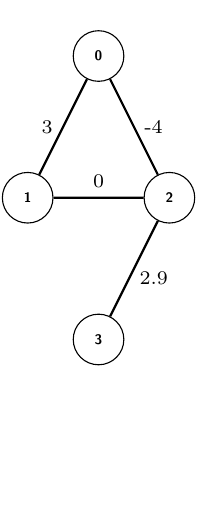
\begin{tikzpicture}[scale=1.8,auto,swap]
                    \node[vertex] (0) at (0.5,3) {0};
                    \node[vertex] (1) at (0,2) {1};
                    \node[vertex] (2) at (1,2) {2};
                    \node[vertex] (3) at (0.5,1) {3};

                    \path[edge] (0) -- node[weight,left] {3} (1);
                    \path[edge] (0) -- node[weight,right] {-4} (2);
                    \path[edge] (1) -- node[weight,above] {0} (2);
                    \path[edge] (2) -- node[weight,right,pos=0.6] {2.9} (3);

                    \pgfresetboundingbox
                    \path [use as bounding box] (0,0) rectangle (1,3.2);
                \end{tikzpicture}
            \end{figure}
        \end{column}%
    \end{columns}
\end{frame}

\begin{frame}[plain,fragile]{Weighted graphs}
    \begin{columns}[T]
        \begin{column}{.4\textwidth}
            \begin{minted}[fontsize=\footnotesize]{cpp}
vector<edge> adj[4];

adj[0].push_back(edge(0, 1, 3));
adj[0].push_back(edge(0, 2, -4));

adj[1].push_back(edge(1, 0, 3));
adj[1].push_back(edge(1, 2, 0));

adj[2].push_back(edge(2, 0, -4));
adj[2].push_back(edge(2, 1, 0));
adj[2].push_back(edge(2, 3, 2.9));

adj[3].push_back(edge(3, 2, 2.9));

            \end{minted}
        \end{column}%
        \hfill%
        \begin{column}{.6\textwidth}
            \begin{figure}
                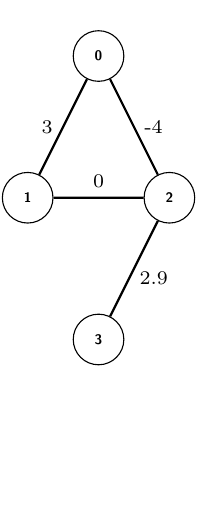
\begin{tikzpicture}[scale=1.8,auto,swap]
                    \node[vertex] (0) at (0.5,3) {0};
                    \node[vertex] (1) at (0,2) {1};
                    \node[vertex] (2) at (1,2) {2};
                    \node[vertex] (3) at (0.5,1) {3};

                    \path[edge] (0) -- node[weight,left] {3} (1);
                    \path[edge] (0) -- node[weight,right] {-4} (2);
                    \path[edge] (1) -- node[weight,above] {0} (2);
                    \path[edge] (2) -- node[weight,right,pos=0.6] {2.9} (3);

                    \pgfresetboundingbox
                    \path [use as bounding box] (0,0) rectangle (1,3.2);
                \end{tikzpicture}
            \end{figure}
        \end{column}%
    \end{columns}
\end{frame}

\section*{Minimum spanning trees}

\begin{frame}[plain]{Minimum spanning tree}
    \begin{itemize}
        \item We have an undirected weighted graph
        \item The vertices along with a subset of the edges in the graph is called a spanning tree if
            \begin{itemize}
                \item it forms a tree (i.e.\ does not contain a cycle) and
                \item the tree spans all vertices (all vertices can reach all other vertices)
            \end{itemize}
        \vspace{10pt}
        \item The weight of a spanning tree is the sum of the weights of the edges in the subset
        \vspace{10pt}
        \item We want to find a minimum spanning tree
    \end{itemize}
\end{frame}

\begin{frame}[plain]{Minimum spanning tree}
    \begin{itemize}
        \item This can model many things, the cheapest way to connect a set of objects is one of them
        \item For some graph problems we can remove everything but a spanning tree to simplify calculations
        \item Note however that it does not have to be unique, but the minimum weight is unique
    \end{itemize}
\end{frame}

\begin{frame}[plain]{Minimum spanning tree}
    \begin{itemize}
        \item Several greedy algorithms work
        \vspace{10pt}
        \item Go through the edges in the graph in increasing order of weight
        \item Greedily pick an edge if it doesn't form a cycle (Union-Find can be used to keep track of when we would get a cycle)
        \item When we've gone through all edges, we have a minimum spanning tree
        \vspace{10pt}
        \item This is Kruskal's algorithm
        \item Time complexity is $O(E \log E)$
    \end{itemize}
\end{frame}

\begin{frame}[plain]{Example}
    \begin{center}
        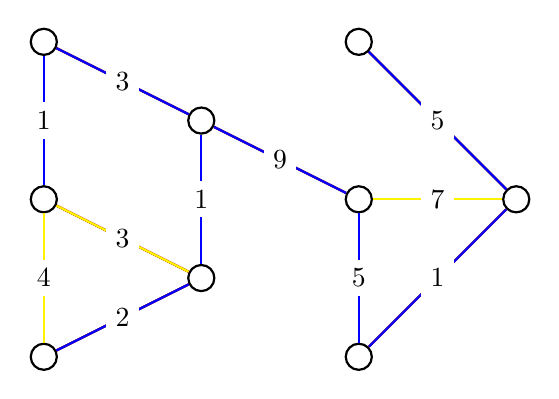
\begin{tikzpicture}
            \node[draw, circle, thick] (1) at (2,0) {};
            \node[draw, circle, thick] (2) at (2,2) {};
            \node[draw, circle, thick] (3) at (2,-2) {};
            \node[draw, circle, thick] (4) at (4,1) {};
            \node[draw, circle, thick] (5) at (4,-1) {};
            \node[draw, circle, thick] (6) at (6,0) {};
            \node[draw, circle, thick] (7) at (6,2) {};
            \node[draw, circle, thick] (8) at (6,-2) {};
            \node[draw, circle, thick] (9) at (8,0) {};

            \onslide<all:1> { \path[draw, thick] (1) -- (2); }
            \onslide<all:2> { \path[draw, thick, red] (1) -- (2); }
            \onslide<all:3-24> { \path[draw, thick, blue] (1) -- (2); }
            \node[fill = white] at (2,1) {$1$};

            \onslide<all:1-9> { \path[draw, thick] (2) -- (4); }
            \onslide<all:10> { \path[draw, thick, red] (2) -- (4); }
            \onslide<all:11-> { \path[draw, thick, blue] (2) -- (4); }
            \node[fill = white] at (3,1.5) {$3$};

            \onslide<all:1-3> { \path[draw, thick] (4) -- (5); }
            \onslide<all:4> { \path[draw, thick, red] (4) -- (5); }
            \onslide<all:5-> { \path[draw, thick, blue] (4) -- (5); }
            \node[fill = white] at (4,0) {$1$};

            \onslide<all:1-7> { \path[draw, thick] (3) -- (5); }
            \onslide<all:8> { \path[draw, thick, red] (3) -- (5); }
            \onslide<all:9-> { \path[draw, thick, blue] (3) -- (5); }
            \node[fill = white] at (3,-1.5) {$2$};

            \onslide<all:1-13> { \path[draw, thick] (1) -- (3); }
            \onslide<all:14> { \path[draw, thick, red] (1) -- (3); }
            \onslide<all:15-23> { \path[draw, thick, yellow] (1) -- (3); }
            \onslide<all:1-23> { \node[fill = white] at (2,-1) {$4$}; }

            \onslide<all:1-21> { \path[draw, thick] (4) -- (6); }
            \onslide<all:22> { \path[draw, thick, red] (4) -- (6); }
            \onslide<all:23-> { \path[draw, thick, blue] (4) -- (6); }
            \node[fill = white] at (5,0.5) {$9$};

            \onslide<all:1-15> { \path[draw, thick] (6) -- (8); }
            \onslide<all:16> { \path[draw, thick, red] (6) -- (8); }
            \onslide<all:17-> { \path[draw, thick, blue] (6) -- (8); }
            \node[fill = white] at (6,-1) {$5$};

            \onslide<all:1-5> { \path[draw, thick] (8) -- (9); }
            \onslide<all:6> { \path[draw, thick, red] (8) -- (9); }
            \onslide<all:7-> { \path[draw, thick, blue] (8) -- (9); }
            \node[fill = white] at (7,-1) {$1$};

            \onslide<all:1-17> { \path[draw, thick] (7) -- (9); }
            \onslide<all:18> { \path[draw, thick, red] (7) -- (9); }
            \onslide<all:19-> { \path[draw, thick, blue] (7) -- (9); }
            \node[fill = white] at (7,1) {$5$};

            \onslide<all:1-19> { \path[draw, thick] (6) -- (9); }
            \onslide<all:20> { \path[draw, thick, red] (6) -- (9); }
            \onslide<all:21-23> { \path[draw, thick, yellow] (6) -- (9); }
            \onslide<all:1-23> { \node[fill = white] at (7,0) {$7$}; }

            \onslide<all:1-11> { \path[draw, thick] (1) -- (5); }
            \onslide<all:12> { \path[draw, thick, red] (1) -- (5); }
            \onslide<all:13-23> { \path[draw, thick, yellow] (1) -- (5); }
            \onslide<all:1-23> { \node[fill = white] at (3,-0.5) {$3$}; }
        \end{tikzpicture}
    \end{center}
\end{frame}

\begin{frame}[plain,fragile]{Minimum spanning tree}
    \begin{minted}[fontsize=\scriptsize]{cpp}

bool edge_cmp(const edge &a, const edge &b) {
    return a.weight < b.weight;
}

vector<edge> mst(int n, vector<edge> edges) {
    union_find uf(n);
    sort(edges.begin(), edges.end(), edge_cmp);

    vector<edge> res;
    for (int i = 0; i < edges.size(); i++) {
        int u = edges[i].u,
            v = edges[i].v;

        if (uf.find(u) != uf.find(v)) {
            uf.unite(u, v);
            res.push_back(edges[i]);
        }
    }

    return res;
}
    \end{minted}
\end{frame}

\begin{frame}[plain]{Minimum spanning tree}
    \begin{itemize}
        \item Another one that works is Prim's algorithm
        \item We start with vertex $0$, then grow the tree one vertex at a time
        \item Each time we take the cheapest edge that connects our tree to something not in the tree
        \item This can also be done in $\mathcal{O}(E\log(E))$
        \item For our purposes Kruskal will suffice
    \end{itemize}
\end{frame}

\section*{Single source shortest path}

\begin{frame}[plain]{Shortest paths}
    \begin{itemize}
        \item We have a weighted graph (undirected or directed)
        \item Given two vertices $u,v$, what is the shortest path from $u$ to $v$?
        \vspace{10pt}
        \item If all weights are the same (or 0/1), this can be solved with breadth-first search
        \item Of course, this is usually not the case...
    \end{itemize}
\end{frame}

\begin{frame}[plain]{Shortest paths}
    \begin{itemize}
        \item There are many known algorithms to find shortest paths
        \item Like breadth-first search, these algorithms usually find the shortest paths from a given start vertex to all other vertices
        \vspace{5pt}
        \item We will look at Dijkstra's algorithm, the Bellman-Ford algorithm and the Floyd-Warshall algorithm
    \end{itemize}
\end{frame}

\begin{frame}[plain]{Shortest paths}
    \begin{itemize}
        \item We will start with the simplest case, where no weights are negative and we want the distance from a particular vertex to the other ones
        \item Why no negative weights? Well if there is a cycle with negative weight on the way to our destination there is no shortest path! You can always go a "shorter" way by cycling around the negative cycle an extra time
        \item In principle Dijkstra is not so dissimilar from BFS
    \end{itemize}
\end{frame}

\begin{frame}[plain]{Shortest paths}
    \begin{itemize}
        \item In BFS the next item in our queue was always the closest one to the source vertex we had not processed yet
        \item In Dijkstra's algorithm we have to do some extra work to ensure this is the case
        \item We use a min-heap, so that the next vertex we pick is always the closest unprocessed one
    \end{itemize}
\end{frame}

\begin{frame}[plain]{Shortest paths}
    \begin{itemize}
        \item We initialize the source vertex to distance $0$, others to $\infty$
        \item We then at any point take the closest vertex $v$ that we haven't processed
        \item We then check all edges adjacent to $v$ and update the distance to the neighbours
        \item We then mark $v$ as done and don't check it again
        \item Note that if all weights are one this will just do the same things as BFS
    \end{itemize}
\end{frame}

\begin{frame}[plain]{Example}
    \begin{center}
        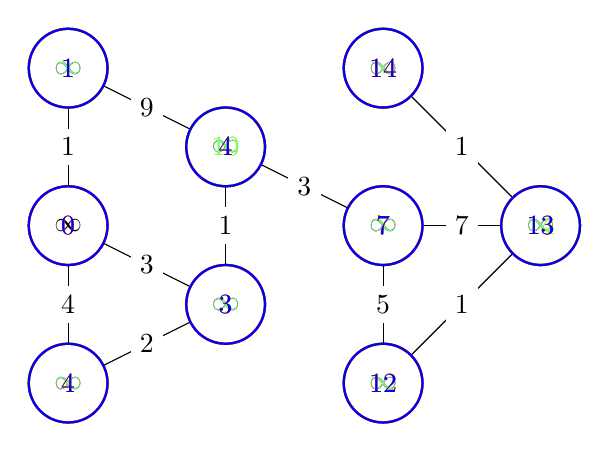
\begin{tikzpicture}
            \onslide<all:1>{\node[draw, circle, thick, minimum size = 1cm] (1) at (2,0) {$\infty$};}
            \onslide<all:2>{\node[draw, circle, thick, minimum size = 1cm, yellow] (1) at (2,0) {$0$};}
            \onslide<all:3-8>{\node[draw, circle, thick, minimum size = 1cm, red] (1) at (2,0) {$0$};}
            \onslide<all:9->{\node[draw, circle, thick, minimum size = 1cm, blue] (1) at (2,0) {$0$};}

            \onslide<all:1-3>{\node[draw, circle, thick, minimum size = 1cm] (2) at (2,2) {$\infty$};}
            \onslide<all:4>{\node[draw, circle, thick, minimum size = 1cm, green] (2) at (2,2) {$\infty$};}
            \onslide<all:5-7>{\node[draw, circle, thick, minimum size = 1cm, green] (2) at (2,2) {$1$};}
            \onslide<all:8-9>{\node[draw, circle, thick, minimum size = 1cm, yellow] (2) at (2,2) {$1$};}
            \onslide<all:10-13>{\node[draw, circle, thick, minimum size = 1cm, red] (2) at (2,2) {$1$};}
            \onslide<all:14->{\node[draw, circle, thick, minimum size = 1cm, blue] (2) at (2,2) {$1$};}

            \onslide<all:1-3>{\node[draw, circle, thick, minimum size = 1cm] (3) at (2,-2) {$\infty$};}
            \onslide<all:4-6>{\node[draw, circle, thick, minimum size = 1cm, green] (3) at (2,-2) {$\infty$};}
            \onslide<all:7>{\node[draw, circle, thick, minimum size = 1cm, green] (3) at (2,-2) {$4$};}
            \onslide<all:8-15>{\node[draw, circle, thick, minimum size = 1cm, yellow] (3) at (2,-2) {$4$};}
            \onslide<all:16-17>{\node[draw, circle, thick, minimum size = 1cm, green] (3) at (2,-2) {$4$};}
            \onslide<all:18-24>{\node[draw, circle, thick, minimum size = 1cm, yellow] (3) at (2,-2) {$4$};}
            \onslide<all:25>{\node[draw, circle, thick, minimum size = 1cm, red] (3) at (2,-2) {$4$};}
            \onslide<all:26->{\node[draw, circle, thick, minimum size = 1cm, blue] (3) at (2,-2) {$4$};}

            \onslide<all:1-10>{\node[draw, circle, thick, minimum size = 1cm] (4) at (4,1) {$\infty$};}
            \onslide<all:11>{\node[draw, circle, thick, minimum size = 1cm, green] (4) at (4,1) {$\infty$};}
            \onslide<all:12>{\node[draw, circle, thick, minimum size = 1cm, green] (4) at (4,1) {$10$};}
            \onslide<all:13-15>{\node[draw, circle, thick, minimum size = 1cm, yellow] (4) at (4,1) {$10$};}
            \onslide<all:16>{\node[draw, circle, thick, minimum size = 1cm, green] (4) at (4,1) {$10$};}
            \onslide<all:17>{\node[draw, circle, thick, minimum size = 1cm, green] (4) at (4,1) {$4$};}
            \onslide<all:18-19>{\node[draw, circle, thick, minimum size = 1cm, yellow] (4) at (4,1) {$4$};}
            \onslide<all:20-23>{\node[draw, circle, thick, minimum size = 1cm, red] (4) at (4,1) {$4$};}
            \onslide<all:24->{\node[draw, circle, thick, minimum size = 1cm, blue] (4) at (4,1) {$4$};}

            \onslide<all:1-3>{\node[draw, circle, thick, minimum size = 1cm] (5) at (4,-1) {$\infty$};}
            \onslide<all:4-5>{\node[draw, circle, thick, minimum size = 1cm, green] (5) at (4,-1) {$\infty$};}
            \onslide<all:6-7>{\node[draw, circle, thick, minimum size = 1cm, green] (5) at (4,-1) {$3$};}
            \onslide<all:8-14>{\node[draw, circle, thick, minimum size = 1cm, yellow] (5) at (4,-1) {$3$};}
            \onslide<all:15-18>{\node[draw, circle, thick, minimum size = 1cm, red] (5) at (4,-1) {$3$};}
            \onslide<all:19->{\node[draw, circle, thick, minimum size = 1cm, blue] (5) at (4,-1) {$3$};}

            \onslide<all:1-20>{\node[draw, circle, thick, minimum size = 1cm] (6) at (6,0) {$\infty$};}
            \onslide<all:21>{\node[draw, circle, thick, minimum size = 1cm, green] (6) at (6,0) {$\infty$};}
            \onslide<all:22>{\node[draw, circle, thick, minimum size = 1cm, green] (6) at (6,0) {$7$};}
            \onslide<all:23-26>{\node[draw, circle, thick, minimum size = 1cm, yellow] (6) at (6,0) {$7$};}
            \onslide<all:27-31>{\node[draw, circle, thick, minimum size = 1cm, red] (6) at (6,0) {$7$};}
            \onslide<all:32->{\node[draw, circle, thick, minimum size = 1cm, blue] (6) at (6,0) {$7$};}

            \onslide<all:1-38>{\node[draw, circle, thick, minimum size = 1cm] (7) at (6,2) {$\infty$};}
            \onslide<all:39>{\node[draw, circle, thick, minimum size = 1cm, green] (7) at (6,2) {$\infty$};}
            \onslide<all:40>{\node[draw, circle, thick, minimum size = 1cm, green] (7) at (6,2) {$14$};}
            \onslide<all:41-42>{\node[draw, circle, thick, minimum size = 1cm, yellow] (7) at (6,2) {$14$};}
            \onslide<all:43>{\node[draw, circle, thick, minimum size = 1cm, red] (7) at (6,2) {$14$};}
            \onslide<all:44->{\node[draw, circle, thick, minimum size = 1cm, blue] (7) at (6,2) {$14$};}

            \onslide<all:1-27>{\node[draw, circle, thick, minimum size = 1cm] (8) at (6,-2) {$\infty$};}
            \onslide<all:28>{\node[draw, circle, thick, minimum size = 1cm, green] (8) at (6,-2) {$\infty$};}
            \onslide<all:29-30>{\node[draw, circle, thick, minimum size = 1cm, green] (8) at (6,-2) {$12$};}
            \onslide<all:31-32>{\node[draw, circle, thick, minimum size = 1cm, yellow] (8) at (6,-2) {$12$};}
            \onslide<all:33-36>{\node[draw, circle, thick, minimum size = 1cm, red] (8) at (6,-2) {$12$};}
            \onslide<all:37->{\node[draw, circle, thick, minimum size = 1cm, blue] (8) at (6,-2) {$12$};}

            \onslide<all:1-27>{\node[draw, circle, thick, minimum size = 1cm] (9) at (8,0) {$\infty$};}
            \onslide<all:28-29>{\node[draw, circle, thick, minimum size = 1cm, green] (9) at (8,0) {$\infty$};}
            \onslide<all:30>{\node[draw, circle, thick, minimum size = 1cm, green] (9) at (8,0) {$14$};}
            \onslide<all:31-33>{\node[draw, circle, thick, minimum size = 1cm, yellow] (9) at (8,0) {$14$};}
            \onslide<all:34>{\node[draw, circle, thick, minimum size = 1cm, green] (9) at (8,0) {$14$};}
            \onslide<all:35>{\node[draw, circle, thick, minimum size = 1cm, green] (9) at (8,0) {$13$};}
            \onslide<all:36-37>{\node[draw, circle, thick, minimum size = 1cm, yellow] (9) at (8,0) {$13$};}
            \onslide<all:38-41>{\node[draw, circle, thick, minimum size = 1cm, red] (9) at (8,0) {$13$};}
            \onslide<all:42->{\node[draw, circle, thick, minimum size = 1cm, blue] (9) at (8,0) {$13$};}

            \path[draw] (1) -- (2); \node[fill = white] at (2,1) {$1$};
            \path[draw] (2) -- (4); \node[fill = white] at (3,1.5) {$9$};
            \path[draw] (4) -- (5); \node[fill = white] at (4,0) {$1$};
            \path[draw] (3) -- (5); \node[fill = white] at (3,-1.5) {$2$};
            \path[draw] (1) -- (3); \node[fill = white] at (2,-1) {$4$};
            \path[draw] (4) -- (6); \node[fill = white] at (5,0.5) {$3$};
            \path[draw] (6) -- (8); \node[fill = white] at (6,-1) {$5$};
            \path[draw] (8) -- (9); \node[fill = white] at (7,-1) {$1$};
            \path[draw] (7) -- (9); \node[fill = white] at (7,1) {$1$};
            \path[draw] (6) -- (9); \node[fill = white] at (7,0) {$7$};
            \path[draw] (1) -- (5); \node[fill = white] at (3,-0.5) {$3$};
        \end{tikzpicture}
    \end{center}
\end{frame}

\begin{frame}{Implementation detail}
\begin{itemize}
\item There is one thing to watch out for
\item The original version of the algorithm uses a heap where you can update the values as you change them
\item This is not possible in most standard libraries, so we use a trick instead
\item We push a new entry into the heap each time we update the weight to a lower one
\item It is \textbf{very important} to only process an entry on the heap if the weight is correct to avoid repeated calculation when doing this!
\end{itemize}
\end{frame}

\begin{frame}[plain,fragile]{Dijkstra's algorithm}
    \tiny
    \begin{minted}{cpp}
vector<edge> adj[100];
vector<int> dist(100, INF);

void dijkstra(int start) {
    dist[start] = 0;
    priority_queue<pair<int, int>, vector<pair<int, int>>, greater<pair<int, int>>> pq;
    pq.push(make_pair(dist[start], start));

    while (!pq.empty()) {
        int u = pq.top().second;
        int w = pq.top().first;
        pq.pop();
        if(dist[u] != w) continue;

        for (int i = 0; i < adj[u].size(); i++) {
            int v = adj[u][i].v;
            int w = adj[u][i].weight;

            if (w + dist[u] < dist[v]) {
                dist[v] = w + dist[u];
                pq.push(make_pair(dist[v], v));
            }
        }
    }
}
    \end{minted}
\end{frame}

\begin{frame}[plain]{Dijkstra's algorithm}
    \begin{itemize}
    \item For each edge in the graph we might have to push to the heap
    \item We visit each vertex at most once and iterate over its neighbours
        \item Thus the time complexity is $O((V + E) \log E)$
        \vspace{10pt}
        \item Note that this only works for non-negative weights
        \item The correctness relies on the fact that once we are done with a vertex we never have to think about it again, which is not true when we have negative weights
    \end{itemize}
\end{frame}

\section*{Dealing with negative weights}

\begin{frame}[plain]{Negative weights}
    \begin{itemize}
    \item What do we do then when we have negative weights?
    \item We can use the Bellman-Ford algorithm, at the cost of a worse time complexity
    \end{itemize}
\end{frame}

\begin{frame}[plain]{Bellman-Ford}
    \begin{itemize}
    \item It is based on dynamic programming, let $f(v, k)$ be the shortest path from the source $u$ to a vertex $v$ that doesn't use more than $k$ vertices to get there
    \item Then as base cases we get $f(u, 0) = 0$ and $f(v, 0) = \infty$ for $v \neq u$
    \item Otherwise we can look at $f(w, k - 1)$ for some $w$, and add a single extra edge, giving the recurrence
    \[f(v, k) = \min \p{ f(v, k - 1), \min_{x \in N^-(v)} \p{ w(x, v) + f(x, k - 1) } }\]
    \end{itemize}
\end{frame}

\begin{frame}[plain]{Bellman-Ford}
    \begin{itemize}
    \item To implement this efficiently we will make some changes from just a straight-forward DP implementation (but that would work!)
    \item Each $f(v, k)$ depends only on $f(w, k - 1)$ for some different $w$, so we only have to store our current row $k$ and the last one
    \item This essentially gets us the usual implementation of Bellman-Ford
    \end{itemize}
\end{frame}

\begin{frame}[plain]{Example}
    \begin{center}
        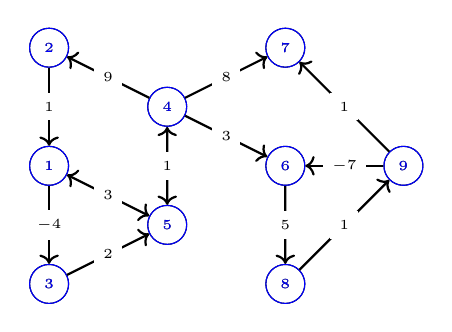
\begin{tikzpicture}[scale = 0.75]
            \onslide<all:2->{\node[draw, circle] (1) at (2, 2) {\tiny $1$};}
            \onslide<all:1>{\node[draw, circle, blue] (1) at (2, 2) {\tiny $1$};}

            \onslide<all:1-3, 6->{\node[draw, circle] (2) at (2, 4) {\tiny $2$};}
            \onslide<all:4, 5>{\node[draw, circle, blue] (2) at (2, 4) {\tiny $2$};}

            \onslide<all:1, 3->{\node[draw, circle] (3) at (2, 0) {\tiny $3$};}
            \onslide<all:2>{\node[draw, circle, blue] (3) at (2, 0) {\tiny $3$};}

            \onslide<all:1-2, 5->{\node[draw, circle] (4) at (4, 3) {\tiny $4$};}
            \onslide<all:3, 4>{\node[draw, circle, blue] (4) at (4, 3) {\tiny $4$};}

            \onslide<all:1, 4->{\node[draw, circle] (5) at (4, 1) {\tiny $5$};}
            \onslide<all:2, 3>{\node[draw, circle, blue] (5) at (4, 1) {\tiny $5$};}

            \onslide<all:1-3, 6-7, 9->{\node[draw, circle] (6) at (6, 2) {\tiny $6$};}
            \onslide<all:4, 5, 8>{\node[draw, circle, blue] (6) at (6, 2) {\tiny $6$};}

            \onslide<all:1-3, 6->{\node[draw, circle] (7) at (6, 4) {\tiny $7$};}
            \onslide<all:4, 5>{\node[draw, circle, blue] (7) at (6, 4) {\tiny $7$};}

            \onslide<all:1-4, 7-8, 10->{\node[draw, circle] (8) at (6, 0) {\tiny $8$};}
            \onslide<all:5, 6, 9>{\node[draw, circle, blue] (8) at (6, 0) {\tiny $8$};}

            \onslide<all:1-5, 8-9, 11->{\node[draw, circle] (9) at (8, 2) {\tiny $9$};}
            \onslide<all:6, 7, 10>{\node[draw, circle, blue] (9) at (8, 2) {\tiny $9$};}



            \path[draw, thick, <-] (1) -- (2); \node[fill = white] at (2,3) {\tiny $1$};
            \path[draw, thick, <-] (2) -- (4); \node[fill = white] at (3,3.5) {\tiny $9$};
            \path[draw, thick, <->] (4) -- (5); \node[fill = white] at (4,2) {\tiny $1$};
            \path[draw, thick, ->] (3) -- (5); \node[fill = white] at (3,0.5) {\tiny $2$};
            \path[draw, thick, ->] (1) -- (3); \node[fill = white] at (2,1) {\tiny $-4$};
            \path[draw, thick, ->] (4) -- (6); \node[fill = white] at (5,2.5) {\tiny $3$};
            \path[draw, thick, ->] (6) -- (8); \node[fill = white] at (6,1) {\tiny $5$};
            \path[draw, thick, ->] (8) -- (9); \node[fill = white] at (7,1) {\tiny $1$};
            \path[draw, thick, <-] (7) -- (9); \node[fill = white] at (7,3) {\tiny $1$};
            \path[draw, thick, <-] (6) -- (9); \node[fill = white] at (7,2) {\tiny $-7$};
            \path[draw, thick, <->] (1) -- (5); \node[fill = white] at (3,1.5) {\tiny $3$};
            \path[draw, thick, ->] (4) -- (7); \node[fill = white] at (5,3.5) {\tiny $8$};
        \end{tikzpicture}
        \vspace{-0.4cm}
        \begin{footnotesize}
            \[
            \begin{array}{r | r r r r r r r r r}
            k & 1 &      2 &      3 &      4 &      5 &      6 &      7 &             8 &             9\\
                \hline
                \onslide<all:1->  {0 & \color{blue} 0 &          \infty &          \infty &          \infty &          \infty &         \infty &          \infty &          \infty &          \infty}\\
                \onslide<all:2->  {1 &              0 &          \infty & \color{blue} -4 &          \infty & \color{blue}  3 &         \infty &          \infty &          \infty &          \infty}\\
                \onslide<all:3->  {2 &              0 &          \infty &              -4 & \color{blue}  4 & \color{blue} -2 &         \infty &          \infty &          \infty &          \infty}\\
                \onslide<all:4->  {3 &              0 & \color{blue} 13 &              -4 & \color{blue} -1 &              -2 & \color{blue} 7 & \color{blue} 12 &          \infty &          \infty}\\
                \onslide<all:5->  {4 &              0 & \color{blue}  8 &              -4 &              -1 &              -2 & \color{blue} 2 & \color{blue}  7 & \color{blue} 12 &          \infty}\\
                \onslide<all:6->  {5 &              0 &               8 &              -4 &              -1 &              -2 &              2 &               7 & \color{blue}  7 & \color{blue} 13}\\
                \onslide<all:7->  {6 &              0 &               8 &              -4 &              -1 &              -2 &              2 &               7 &               7 & \color{blue}  8}\\
                \onslide<all:8->  {7 &              0 &               8 &              -4 &              -1 &              -2 & \color{blue} 1 &               7 &               7 &               8}\\
                \onslide<all:9->  {8 &              0 &               8 &              -4 &              -1 &              -2 &              1 &               7 &  \color{blue} 6 &               8}\\
                \onslide<all:10-> {9 &              0 &               8 &              -4 &              -1 &              -2 &              1 &               7 &               6 &   \color{red} 7}\\
        \end{array}
        \]
        \end{footnotesize}
    \end{center}
\end{frame}

\begin{frame}[plain]{Bellman-Ford}
    \begin{itemize}
    \item How do we read negative cycles from this though?
    \item In a graph with no negative cycles a shortest path visits each vertex at most once
    \item Thus we can simply do $V - 1$ more values of $k$ to see if anything gets shorter
    \item If the distance to $v$ gets shorter then there is a negative cycle on the way to $v$
    \end{itemize}
\end{frame}

\begin{frame}[plain,fragile]{Bellman-Ford algorithm}
    \begin{minted}[fontsize=\footnotesize]{cpp}
vector<edge> adj[100];
vector<int> dist(100, INF);

void bellman_ford(int n, int start) {

    dist[start] = 0;

    for (int i = 0; i < n - 1; i++) {
        for (int u = 0; u < n; u++) {
            for (int j = 0; j < adj[u].size(); j++) {
                int v = adj[u][j].v;
                int w = adj[u][j].weight;
                dist[v] = min(dist[v], w + dist[u]);
            }
        }
    }
}
    \end{minted}
\end{frame}

\begin{frame}[plain]{Bellman-Ford}
    \begin{itemize}
    \item This gets us a $\mathcal{O}(VE)$ algorithm, which is quite a bit slower than Dijkstra
    \item A possible improvement is to store every vertex that received an update for the last $k$ value in a queue, and only checking things they could affect at the next $k$
    \item This is still worst case $\mathcal{O}(VE)$, but in the average case much much faster
    \item This is generally known as the SPFA algorithm (Shortest Path Faster Algorithm)
    \end{itemize}
\end{frame}

\section*{All pairs shortest path}

\begin{frame}[plain]{Bellman-Ford}
    \begin{itemize}
    \item What if we want to get the distance from every vertex to every vertex?
    \item If there are no negative cycles running Dijkstra's from every vertex works pretty well
    \item But for negative cycles running Bellman-Ford $V$ times is pretty slow
    \item Luckily we can get a bulk discount in this case!
    \item This is known as the Floyd-Warshall algorithm
    \end{itemize}
\end{frame}

\begin{frame}[plain]{Floyd-Warshall algorithm}
    \begin{itemize}
        \item We use dynamic programming again.
        \vspace{10pt}
    \item Let $\mathrm{sp}(k, i, j)$ be the shortest path from $i$ to $j$ if we're only allowed to travel through the vertices $0$, \ldots, $k$
        \vspace{5pt}
    \item Base case: $\mathrm{sp}(k, i, j) = 0$ if $i = j$
    \item Base case: $\mathrm{sp}(-1, i, j) = \mathrm{weight}[i][j]$ if $(i,j) \in E$
    \item Base case: $\mathrm{sp}(-1, i, j) = \infty$
        \vspace{5pt}
    \item $\mathrm{sp}(k, i, j) = \mathrm{min} \left\{
	\begin{array}{l}
        \mathrm{sp}(k - 1, i, k) + \mathrm{sp}(k - 1, k, j) \\
        \mathrm{sp}(k - 1, i, j)
	\end{array}
\right.$
    \end{itemize}
\end{frame}

\begin{frame}[plain,fragile]{Floyd-Warshall algorithm}
    \begin{minted}[fontsize=\scriptsize]{cpp}
int dist[1000][1000];
int weight[1000][1000];

void floyd_warshall(int n) {
    for (int i = 0; i < n; i++) {
        for (int j = 0; j < n; j++) {
            dist[i][j] = i == j ? 0 : weight[i][j];
        }
    }

    for (int k = 0; k < n; k++) {
        for (int i = 0; i < n; i++) {
            for (int j = 0; j < n; j++) {
                dist[i][j] = min(dist[i][j], dist[i][k] + dist[k][j]);
            }
        }
    }
}
    \end{minted}
\end{frame}

\begin{frame}[plain]{Floyd-Warshall algorithm}
    \begin{itemize}
\item Computes all-pairs shortest paths
\item Time complexity is clearly $O(n^3)$
\item Very simple to code
\item Though we can do better! By combining everything we did so far and mixing in an algorithm known as Johnson's algorithm, Floyd-Warshall can be beat. But this won't be in the homework (maybe the bonus problems!)
    \end{itemize}
\end{frame}

\end{document}

